\documentclass{article} % For LaTeX2e
% We will use NIPS submission format
\usepackage{nips13submit_e,times}
% for hyperlinks
\usepackage{hyperref}
\usepackage{url}
% For figures
\usepackage{graphicx} 
\usepackage{subfigure} 
% math packages
\usepackage{amsmath}
\usepackage{amsfonts}
\usepackage{amsopn}
\usepackage{ifthen}
\usepackage{natbib}

\title{Project-I by Group CITYNAME}

\author{
Mohammad Emtiyaz Khan\\
EPFL \\
\texttt{emtiyaz@gmail.com} \\
}

% The \author macro works with any number of authors. There are two commands
% used to separate the names and addresses of multiple authors: \And and \AND.
%
% Using \And between authors leaves it to \LaTeX{} to determine where to break
% the lines. Using \AND forces a linebreak at that point. So, if \LaTeX{}
% puts 3 of 4 authors names on the first line, and the last on the second
% line, try using \AND instead of \And before the third author name.

\nipsfinalcopy 

\begin{document}

\maketitle

\begin{abstract}
In this report, we summarize our findings for the demo done on October 23, 2014.
We fit several linear methods to the regression dataset and compare them.
We found that the input matrix is ill-conditioned and therefore ridge regression is prefered over least-squares. It also appears that the linear model is appropriate for this data and predicts the data reasonably well. We also investigated a few feature transformations but found no significant improvements.
\end{abstract}

\section{Data Description}
Our train-data consists of output variables $\mathbf{y}$ and input variables $\mathbf{X}$. We have $N=600$ data examples. Each input vector $\mathbf{x}_n$ is of dimensionality $D=10$. Out of these 10 variables, 8 variables are real valued while 1 variable is binary and 1 variable is categorical with 4 categories.

We also have test-data where we do not observe $\mathbf{y}$. We have $N=600$ test examples. Our goal is to produce predictions for test examples, as well as an approximation of the test-error.

\section{Data visualization and cleaning}
We performed basic exploratory data analysis on our data. Figure \ref{fig:boxplotX} shows distributions of all 10 input variables. As expected the data is not centered, and therefore we normalize the data. Figure \ref{fig:histY} shows the histogram of the output variable. We see that there are two data points which have rather high value of the output variables compared to rest of the data. Since these are only two data points, we remove them from the data (example number 362 and 402).

We also investigated the correlation between output and input variables (plot not shown, since it is not important for our analysis). We found that most of the variables are correlated with the output, confirming the need for a full regression analysis. The third variable did not seem significantly correlated, however this preliminary observation does not suggest removal of this variable from the dataset.

We use a dummy encoding for the categorical variable. The binary variable does not require any dummy encoding. This gives us a total of 14 input variables.

The input matrix $\mathbf{X}$ is rank-deficient with a rank of 6, instead of 10. This implies that we must ``lift" the eigenvalues, using methods such ridge regression.

\begin{figure}[!t]
\center
\subfigure[Boxplot of real-valued $\mathbf{X}$. Data is not centered and therefore we normalize it.]{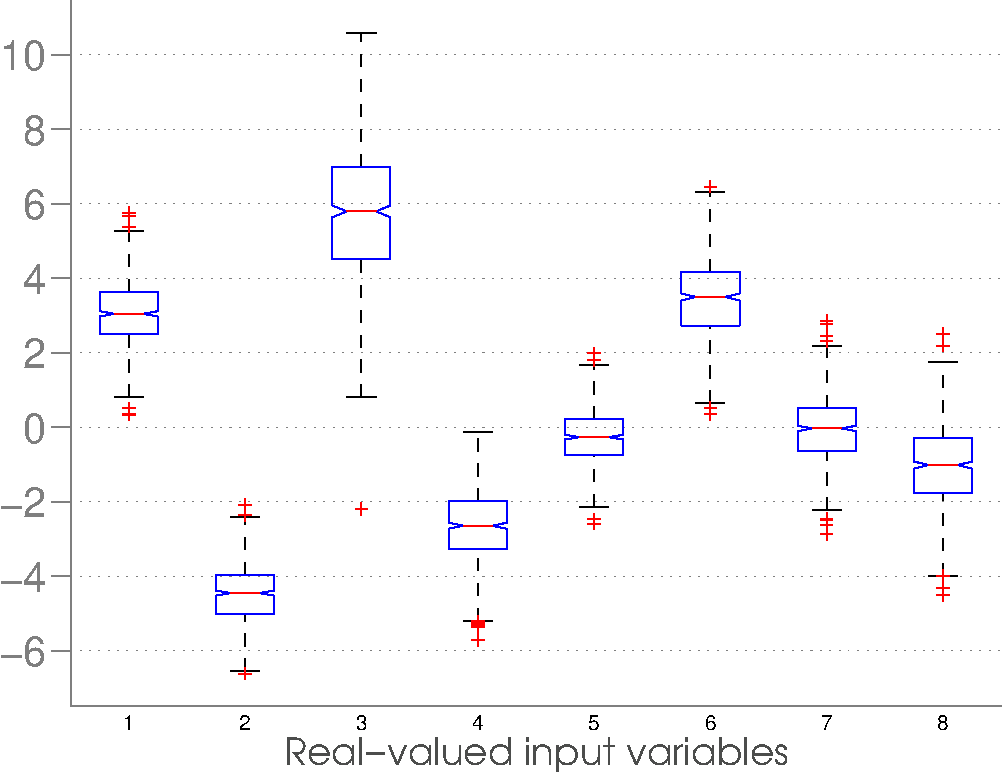
\includegraphics[width=2.5in]{figures/boxplotX.pdf} \label{fig:boxplotX}}
\hfill
\subfigure[Histogram of $\mathbf{y}$. We can clearly see two outliers.]{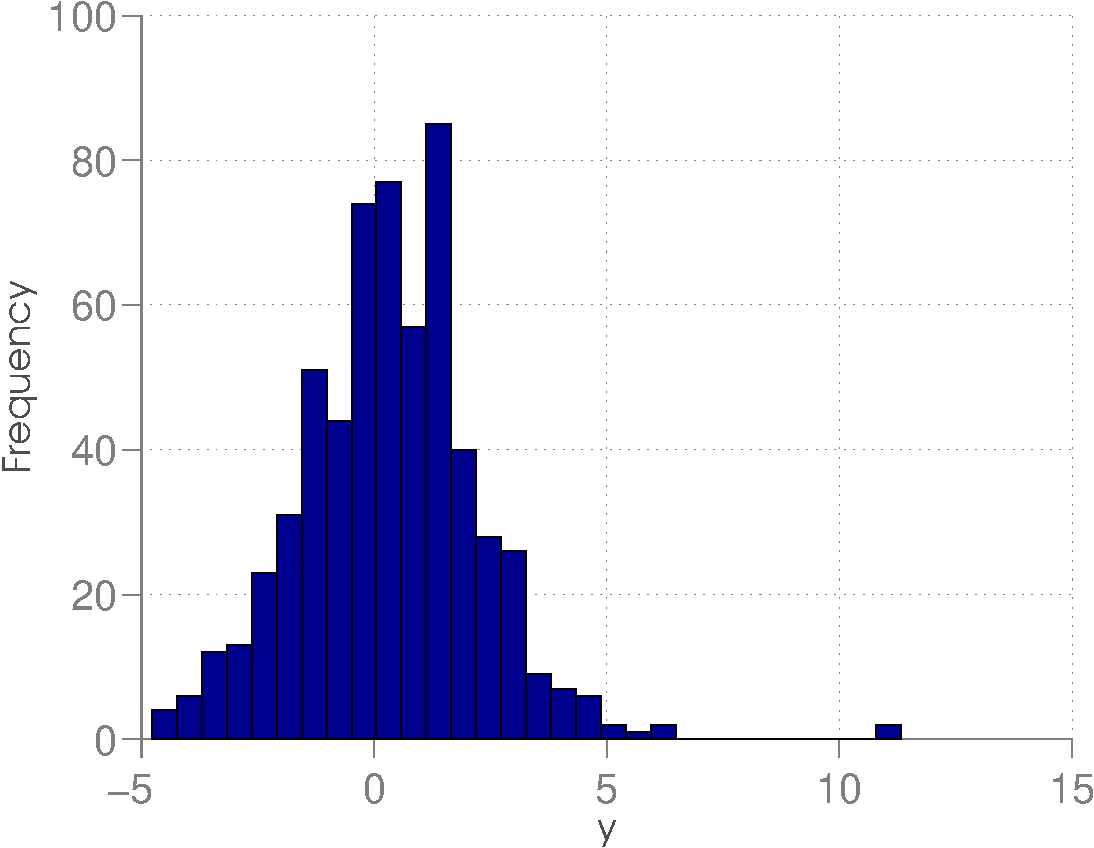
\includegraphics[width=2.5in]{figures/histY.pdf} \label{fig:histY}}
\caption{}
\end{figure}

\section{Ridge regression}
We applied least-squares and ridge regression to this dataset. Since the matrix is ill-conditioned, least-squares is not suitable. Therefore, we report results obtained with ridge regression alone. Note that the improvements using ridge regression were modest and not much lower than that of linear regression, however we do not expect least-squares to work well when there is a lot of testing data available. 

Figure \ref{fig:ridgeCurve} shows the results obtained with ridge regression when we use $50\%$ of the data as test data and rest as training data. We varied the value of $\lambda$ from $10^{-4}$ to $10^3$, choosing total 500 points in between. We can see that there is a small improvement obtained for some values of $\lambda$.

We did experiments to plot a learning curve for this data (see Andrew Ng's notes about the learning curve). We held out 20\% of data as test data and rest as training data. We chose to slowly increase the proportion of data used for training. For each proportion of the training data, we repeated the experiment 30 times to compute the distribution of error. We fit ridge regression to each sampled training set and test it on the same $20\%$ test data. We varied the value of $\lambda$ from $10^{-4}$ to $10^3$, choosing total 500 points in between.

This gives us the learning curve shown in Fig. \ref{fig:learnCurve}. The blue curve shows the train error while red curve shows the test error. We can see that both training and test error converge, with the variance of estimates decreasing as we increase the training data size. There is also a very small gap between the train and test errors, showing that the linear model is a reasonable choice. The small gap exists perhaps because we have only limited test data.

\section{Feature transformations}
We tried several feature transformations. We found that we get a small improvement in performance when we take $\sqrt{|X_{ni}|}$ for all entries of $\mathbf{X}$. We did not check (due to lack of time) whether it matters if we apply this to one variable or all. We performed experiments similar to the last section (although one should really do cross-validation). Values of lambda were kept same as the last section. 

We compare three methods. First is a baseline where we do not use any input variables i.e. mean value of the output. The second method is the ridge regression described in previous section. The third method is ridge regression with a feature transformation. The first method gave RMSE of around 3 which was way worse than the other two methods.

The RMSE for the last two methods are shown in Fig. \ref{fig:summary}. We see that both test and train error decrease, however it appears that the improvement is very little and may not be significant.


\begin{figure}[!h]
\center
\subfigure[Ridge regression for a 50-50 split.]{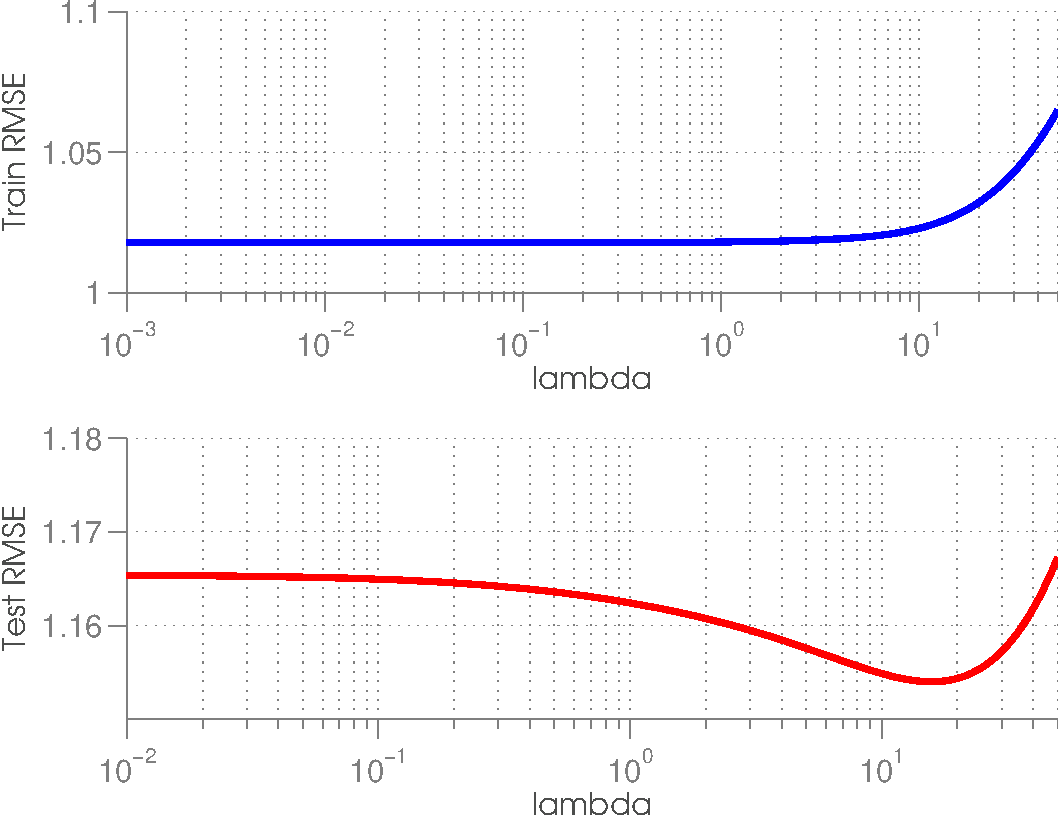
\includegraphics[width=2.5in]{figures/ridgeCurve.pdf} \label{fig:ridgeCurve}}
\hfill
\subfigure[Comparison of ridge regression with and without feature transformation. The improvement is very little and might be insignificant.]{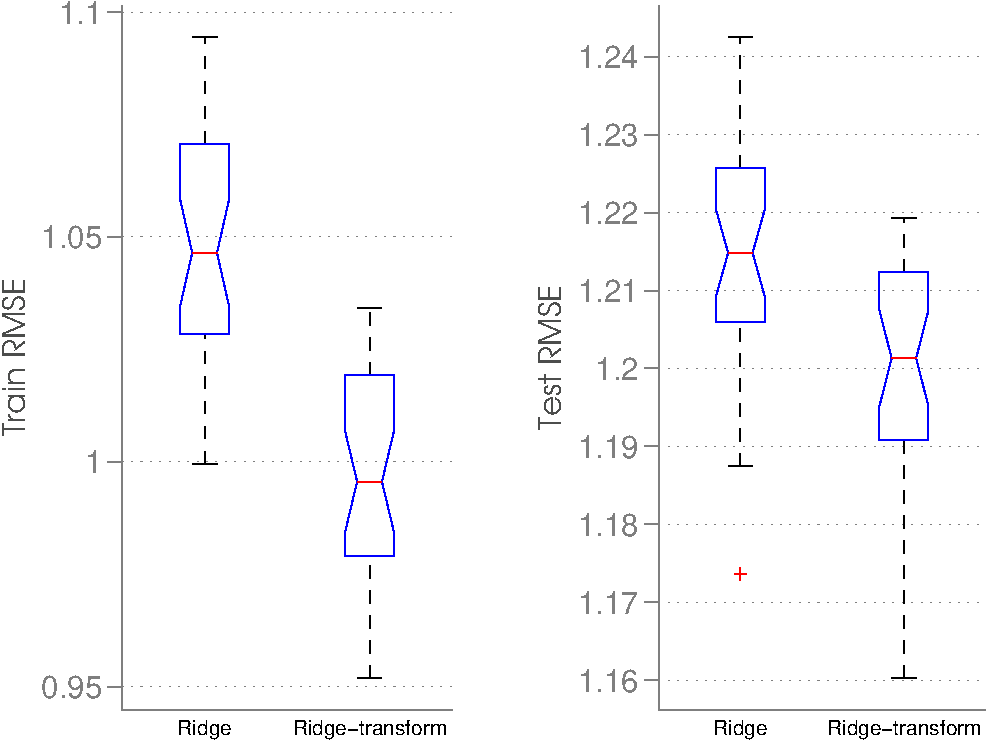
\includegraphics[width=2.7in]{figures/summary.pdf} \label{fig:summary}}
\subfigure[Learning curve. Blue is training data and red is test data.]{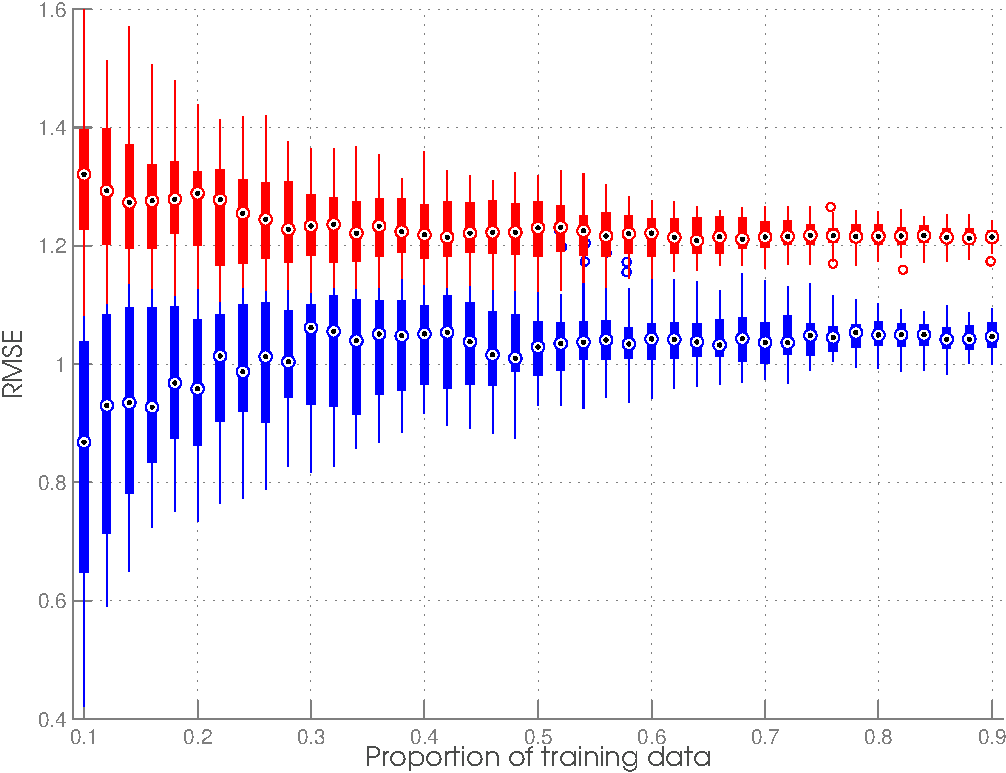
\includegraphics[width=4in]{figures/learningCurve.pdf} \label{fig:learnCurve}}
\caption{}
\end{figure}


\section{Summary}
In this report, we analyzed a regression dataset and found that ridge regression is a reasonable fit. We estimate that the average test error is 1.213 ($\pm$ 0.02). We tried some feature transformation and found that there is a small improvement giving us a test error of around 1.198 ($\pm$ 0.015). This improvement, however, is not significant.


\subsubsection*{Acknowledgments}
We would like to thank Timur for making the dataset for this study, Carlos and Ilija to help conduct the experiments, and all the students who attended the session making it exciting for us. All the code, as well as this report, was written by Emti. 

\subsubsection*{References}

\end{document}
